
\begin{SCfigure}[1][htb]
    \centering
    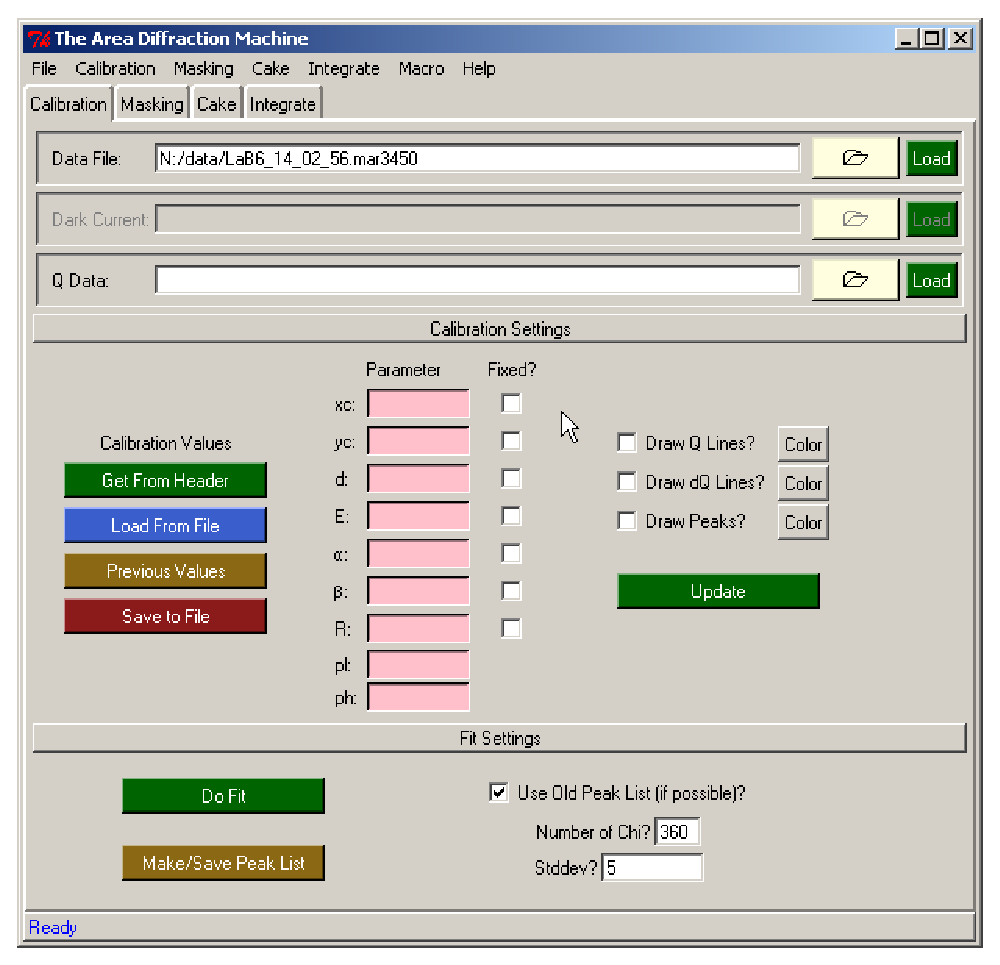
\includegraphics[scale=.75]{figures/calibration_page.eps}
    \caption{A screen shot of the calibration tab to the program.
    This is what you see when you first open up the program. 
    This page allows you to, among other things, load diffraction
    data into the program.`} 
    \label{calibration_page}
\end{SCfigure}



When you first open up the Area Diffraction Machine, you
will be presented with the window shown in 
figure~\ref{calibration_page}. The first thing that you
will probably want to do is load some diffraction data into
the program. To do so, you can see the Data File: input.
You can either type in the filename by hand and push the
load button or click on the folder icon to the side and
use the file selector to pick the file that you want.
Once the file is loaded, you will be presented with
the window shown in figure~\ref{diffraction_data_window}

\begin{SCfigure}[1][htb]
    \centering
    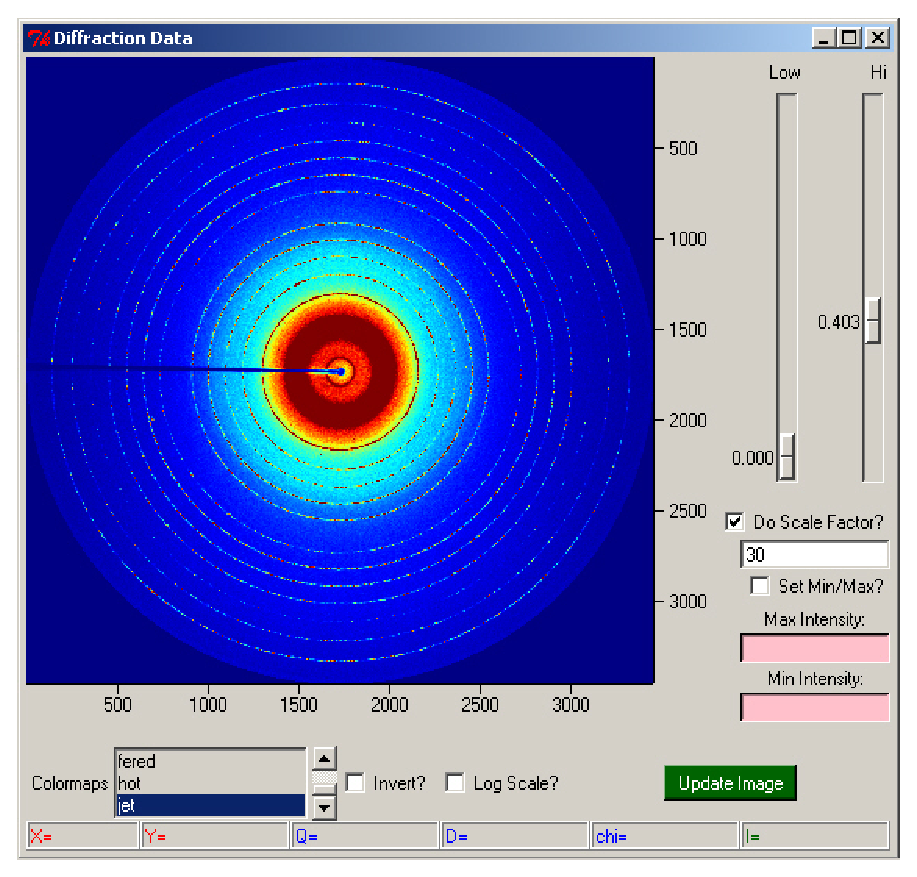
\includegraphics[scale=.75]{figures/diffraction_data_window.eps}
    \caption{A screen shot of the diffraction data window for
    the program. This window will be opened up after a file is 
    loaded. This windows allows you to interact with diffraction 
    data.} 
    \label{diffraction_data_window}
\end{SCfigure}


Once the diffraction data window has opened up, you can use
the window to interact with your diffraction data. With
the window you can
\begin{itemize}
    \item {\em Zoom into the data} - To zoom, left click on
    the data and hold down on the mouse. When you drag the cursor, 
    the program will create a resizing square. When you let go of the
    mouse, the selected square will be used as the outer bound and
    the image will be zoomed into it.
    \item {\em Zoom out of the data} - To unzoom, right click on
    the data.
    \item {\em Pan across the data} - To pan, hold down on shift, than
    right (or left) click on the data and hold down on the mouse. When 
    you move the mouse, the program will pan the image to follow the 
    cursor. When you let go of the mouse, the program will stop panning.
    \item {\em Resize the window} - This will make the diffraction
    image either larger or smaller. To do so, click on the bottom 
    right corner and drag.
    \item {\em Read coordinates for a selected point} - When you
    mouse over the image, the $x$, $y$, $Q$, $\chi$, and $I$
    values for that pixel will be displayed at the bottom of the
    window.
    \item {\em Change the Color Map} - You can use the 
    \gui{Colormaps} selector to change the particular color map that 
    is used to display the data.
    \item {\em Invert the Color Map} - You can use the 
    \gui{Invert?} checkbox to invert the colors of the color map.
    \item {Low \& Hi Pixels} You can use the sliders to the
    right of the image to change the intensity scaling of the
    image. The low value corresponds to the intenisty 
    value\footnote{Technically, what you actually select is what
    percentage of the most intense pixel should be mapped to
    the lowest or highest value in value in the color map.}
    that will be maped to the lowest part of
    the color map and the hi value corresonds to the intensity
    value that will be mapped to the highest part of the color
    map. This feature is useful for making visible only certain
    intensity ranges in teh image.
    \item {\em Log Scaling the Color Map} - By defualt, intensity
    values are linearly mapped to colors using the given color
    map, but you can use the \gui{Log Scale?} checkbox to instead
    apply a log scale mapping of the intensity values to the color
    map.
\end{itemize}


\subsection{File Formats}

The program can load in Mar data: \macroline{.mar3450}, 
\macroline{.mar2300}, and \macroline{.mccd} marccd format.
It can load in standard \macroline{.tiff} data. 
It can load in the ESRF Data Format 
\macroline{.edf}.

The program can only display square data, so whenever non-square
data is loaded in, the program will simply pad out the image until
it is a square with pixels who's intensity is 0. 


\subsection{Loading Multiple Images}

Using the same file input, you can load multiple files into 
the program at the same time. To do this, you can either put multiple
files names into the \gui{Data File:} text input. Each file needs to
be space separated. The input is far to small for this to be very useful,
so it is much easier instead to use the file selector by pushing the
button with the folder on it. When you open the selector up, you can 
simply select multiple files and then load them in.

When several files are loaded at the same time, the program will add
the images together pixel by pixel and work with the combined image.
This can be useful for analyzing one several images all taken of the
same sample. Obviously, the program can only add together files of
the same format.

\subsection{Saving the Diffraction Image}
\index{Save}\index{ESRF Data Format}
You can save the current diffraciton image that you have loaded 
as a popular image format. To save the image, you can go into
the \gui{File} menubar and select the \gui{Save Image} option.

The formats currently allowed are jpg, gif, eps, pdf bmp, png, 
tiff , and the ESRF data format edf.

Because the program will pad any non-sqaure data when
it is loaded to make it square. The program will always save out 
the images as squares. If this is undesriable, the saved images
will need to be cropped using another program.

